
\documentclass[xcolor=pdftex,table,11pt]{beamer}
\usetheme{Warsaw}
\usepackage[utf8]{inputenc}
\usepackage[english]{babel}
\usepackage{amsmath}
\usepackage{amsfonts}
\usepackage{amssymb}
\usepackage{multirow}
\usepackage{siunitx}
\usepackage{listings}
\usepackage{tabulary}
\usepackage[highlightcolor=yellow]{../styles/code}
\author{Informática I - Instituto Unviersitario Areonáutico}
\title{Introducción a los algoritmos}

\usepackage{booktabs}
\usepackage{longtable}
\newcommand*{\thead}[1]{\multicolumn{1}{c}{\bfseries #1}}


%\setbeamercovered{transparent} 
%\setbeamertemplate{navigation symbols}{} 
%\logo{} 
%\institute{} 
%\date{} 
%\subject{} 
\begin{document}


\begin{frame}
\titlepage
\end{frame}

\begin{frame}
\tableofcontents
\end{frame}

\begin{frame}{¿Qué son los algoritmos?}
\begin{block}{Según la RAE}
         Conjunto ordenado y finito de operaciones que permite hallar la solución a un problema.
    \end{block}
 
 \begin{block}{Según Deitel}
         Es el procedimiento para resolver un problema en términos de las acciones a ejecutar y el órden en el cual se llevan a cabo dichas acciones.
    \end{block}
    
\begin{block}{¿Cómo está compuesto un algoritmo?}
   \begin{itemize}
   \item Entrada
   \item Procesamiento
   \item Salida
   \end{itemize}
\end{block}


\end{frame}



\begin{frame}{Ejemplos de algoritmos}

\begin{block}{Preparar una taza de té}
   \begin{itemize}
   \item Entrada: agua, saquito de té, taza
   \item Salida: té caliente
   \item Procedimiento: 
   \begin{itemize}
   \item[]<1-> Inicio del algoritmo

   \begin{itemize}
   
     	\item<1-> Poner el agua fría dentro de la pava
     	 \item<2-> Encender el fuego 
     	 \item<3-> Poner la pava sobre el fuego
   		\item<4-> Esperar que el agua se caliente
   		\item<5-> Poner el saquito de té en la taza
 		\item<6-> Agregar el agua caliente
 		\item<7-> Apagar el fuego
 		\item<8-> Esperar un minuto
 		
   \end{itemize}
 \item[]<9-> Fin del algoritmo

	\end{itemize}
\end{itemize}

\end{block}


\end{frame}



\begin{frame}{Ejemplo de algoritmos}

\begin{block}{Calcular la distancia recorrida por un móvil que se movió en MRUV}
    \begin{equation}\label{eq:d_mruv}
            x(t) = V_0 t + \frac{1}{2}  a  t^2  
    \end{equation}
   \begin{itemize}
   \item Entrada: velocidad inicial, tiempo recorrido, aceleración
   \item Salida: distancia recorrida
   \item Procedimiento: 
   \begin{itemize}
   \item[]<1-> Inicio del algoritmo

   \begin{itemize}
   
     	\item<1-> Ingresar la velocidad inicial del movil
        \item<2-> Ingresar el tiempo de desplazamiento
 		\item<3-> Ingresar la aceleración
 		\item<4-> Aplicar la fórmula \ref{eq:d_mruv}
 		\item<5-> Informar la distancia
   \end{itemize}
 \item[]<6-> Fin del algoritmo

	\end{itemize}
\end{itemize}

\end{block}


\end{frame}



\begin{frame}{Pseudocódigo}
\begin{block}{Definición}

El pseudocódigo es un lenguaje artificial e informal que ayuda a los programadores a desarrollar y probar algoritmos.
\end{block}
\begin{block}{Ejemplo para calcular el volumen de una esfera}

 \begin{itemize}
   \item[]<1-> Inicio del algoritmo

   \begin{itemize}
   
     	\item<1-> Imprimir: Ingrese el radio de la esfera
        \item<2-> Leer: radio
 		\item<3-> $v_{esfera} =\frac{4}{3}  \pi  r^3  $
 		\item<4-> Imprimir: "El volumen de la esfera es $v_{esfera}$"
   \end{itemize}
 \item[]<5-> Fin del algoritmo

	\end{itemize}
\end{block}


\end{frame}

\begin{frame}{Diagrama de flujo}
\begin{columns}
\column{0.5\textwidth}
 \begin{itemize}
   
     	\item<1-> Es la representación gráfica de un algoritmo
        \item<2-> Se dibujan mediante símbolos de propósito especial: rectángulos, rombos, olvalos y círculos entre otros
 		\item<3-> Estos símbolos se conectan mediantes flechas llamadas \textbf{líneas de flujo}
 		\item<4-> \textbf{Tienen un solo punto de inicio y fin}.
   \end{itemize}
\column{0.5\textwidth}
 \begin{figure}
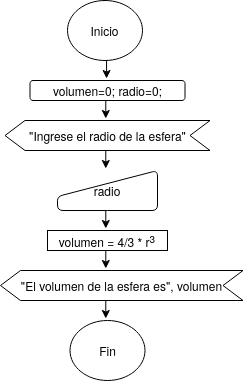
\includegraphics[scale=0.4]{../img/exported/volumen_esfera.png}
\caption{Diagrama de flujo para el cálculo del volúmen de una esfera}
\end{figure}
\end{columns}
\end{frame}




\begin{frame} {Tipos de datos en C}
El lenguaje de programación C es \textbf{fuertemente tipado}, es decir que cada vez que se necesite declarar u operar con una variable, se debe definir y tener presente el tipo de la misma. \\
Nota: ver los tipos de datos \textit{Unsigned}
\begin{table}
\begin{tabular}{l | c | c | c | l }
Tipo de dato & Descripción & Rango  \\
\hline \hline
short & Valor entero de 2 bytes & $-2^{16}$ a $2^{16} -1 $\\ 
int & 	Valor entero de 4 bytes & $-2^{32}$ a $2^{32} -1 $\\ 
long & 	Valor entero de 8 bytes & $-2^{64}$ a $2^{64} -1 $\\ 
char & Caracteres ASCII & $-128 $ a $127$\\ 
float & Valor decimal de 4 bytes & $\num{3.4e-38} $ a $\num{3.4e-38}$\\ 
double & Valor decimal de 8 bytes & $\num{1.7e-308} $ a $\num{1.7e-308}$\\ 
bool & Valor binario &True o False\\ 
void & Tipo de dato nulo &\\ 
 string & Cadena de char  &\\ 
\end{tabular}
\caption{Tipos de datos en C}

\end{table}

\end{frame}


\begin{frame}[allowframebreaks] {Entrada y salida de datos}
Para imprimir por pantalla o ingresar datos a un programa en C, se debe informar \textbf{expresamente} el tipo de dato que se espera imprimir y/o recibir.
Esto se realiza mediante el uso de \textbf{especificadores de formato}.

\begin{table}
\begin{tabular}{l | c | l }
Tipo de dato & Especificador de formato \\
\hline \hline
short & $\%hd$ \\ 
int & 	$\%d$ \\ 
long & 	$\%li$ \\ 
char & $\%c$\\ 
float & $\%f$ \\ 
double & $\%lf$\\ 
\end{tabular}
\caption{Especificadores de formato en C}
\end{table}
 \begin{block}{Scanf}
Es una función de la librería de entrada/salida de C que permite tomar información desde el teclado.\\ 

Sintaxis: scanf("especificador de formato", $\&$variable); \\ 
Ejemplo	: scanf("$\%d$", $\&$edad); \\ 
    \end{block}

 \begin{block}{Printf}
Es una función de la librería de entrada/salida de C que permite imprimir información por pantalla.\\ 
Sintaxis: printf("especificador de formato", variable); \\ 
Ejemplo: printf("Su edad es: " $\%d$ , edad);
    \end{block}
    

Nota: para estos ejemplos se supone que la variable se ha declarado de tipo int. Ver ejemplos siguientes.
\codesetstylefrombeamer
\cppfile{../../c/src/1-0_data_types_edad_peso.c}
\end{frame}


\begin{frame}{Operaciones aritméticas en C}
\begin{table}
\begin{tabular}{p{22mm} | p{22mm} | p{22mm} | p{22mm} | p{22mm} }
Operación en C & Operador aritmético & Expresión algebraica & Expresión algebraica\\
\hline \hline 
Adición 		& 	$+$   & $num + 10$ 	 	& $num + 10$ \\
Sustracción 	& 	$-$	  & $num - 10$ 	 	& $num + 10$ \\
Multiplicación 	& 	$*$   & $num.10$  		& $num * 10$ \\
División 		& 	$/$	  & $num / 10$  	& $num / 10$ \\
Resto 			& 	$\%$  & $num mod 10$  	& $num \% 10$ \\ 

\end{tabular}
\caption{Especificadores de formato en C}
\end{table}




\end{frame}


\begin{frame}{Precedencia de operadores}
El lenguaje C evalúa las expresiones aritméticas en una secuencia precisa, por lo general son las mismas que aplicaríamos en el álgebra:\\

\begin{enumerate}
\item Las operaciones de multiplicación, división y módulo se resuelven primero. Si en una misma operación aparecen varias de ellas, se resuelven de izquierda a derecha

\item Las operaciones de suma y resta se aplican después. Si hubiese varias de estas, C separará en términos al igual que se haría en el álgebra

\item Luego de resueltas todas las operaciones, se procede a la asignación

\end{enumerate}
\end{frame}

\begin{frame}{Precedencia de operadores: ejemplo}


 \begin{block}{Ecuación de una recta en forma algebraica}
\begin{equation}
y(x) = a x + b
\end{equation}
    \end{block}
    

 \begin{block}{Ecuación de una recta en C}
\begin{equation}
y = a * x + b
\end{equation}


  \end{block}

 \begin{block}{Precedencia de operadores}
 \begin{enumerate}
\item Operación $a * x$
\item Operación $+b$
\item Asignación del resultado a la variable $y$
\end{enumerate}
  \end{block}
\end{frame}
\begin{frame}{Precedencia de operadores: ejemplo en C}
\codesetstylefrombeamer
\cppfile{../../c/src/1-1_presedencia_operadores.c}
\end{frame}

hola, esto es lo que estoy probando 


\end{document}